%\documentclass[11pt,letter9paper]{article}
\documentclass{llncs}
\pagestyle{plain}

\usepackage{amsfonts,amsmath,amssymb}
\usepackage[backend=bibtex,giveninits=true,style=numeric,maxnames=6]{biblatex}
\bibliography{references}
\renewcommand*{\bibfont}{\footnotesize}
%\usepackage{booktabs}
%\usepackage[margin=1.5cm,footskip=30pt,includefoot]{geometry} % messes with LNCS margin formatting
\usepackage[utf8]{inputenc}
\usepackage[colorlinks=true,citecolor=black,linkcolor=black,urlcolor=black]{hyperref}
\usepackage{mathtools}
\usepackage{xspace}
\usepackage{xcolor}
\usepackage{comment}
\usepackage{multirow}
\DeclareMathAlphabet{\mathsc}{OT1}{cmr}{m}{sc}
\usepackage{bm}
\usepackage{framed}
%\usepackage{siunitx}
\usepackage[capitalise]{cleveref}
\usepackage{enumitem}
%\usepackage{microtype} % fixes overhangs
\usepackage{ifthen} % \ifthenelse for figures
\usepackage{float} % to make figures not go to the end
%\usepackage{dashbox} % dashed boxes to highlight where FROST1 and FROST 2 differ
%\usepackage{soul}
\usepackage{comment}
\usepackage{pifont} % to get \xmark

\usepackage{graphicx}
\graphicspath{ {./images/} }

\usepackage[
%lambda, % or n
%advantage,
%operators,
%sets,
%adversary,
%landau,
%probability,
%notions,
%logic,
%ff,
%mm,
%primitives,
%events,
%complexity,
%oracles,
%asymptotics,
%keys
]{cryptocode}

\usepackage{array}
\newcommand{\PreserveBackslash}[1]{\let\temp=\\#1\let\\=\temp}
\newcolumntype{C}[1]{>{\PreserveBackslash\centering}p{#1}}
\newcolumntype{R}[1]{>{\PreserveBackslash\raggedleft}p{#1}}
\newcolumntype{L}[1]{>{\PreserveBackslash\raggedright}p{#1}}
\def\arraystretch{1.15}

%\usepackage{ulem} % strikethrough text but makes references overhang so removed

% From CTZ Paper
\usepackage{setspace} % for \setstretch

%%% Delete if include llncs
%\newtheorem{definition}{Definition}[section]
%\newtheorem{theorem}{Theorem}
%\newtheorem{lemma}{Lemma}
\newtheorem{assumption}{Assumption}

%\setcounter{tocdepth}{3}

\usepackage{afterpage} % for \setstretch
\usepackage{booktabs}

\title{FROST Submission}
\date{\today}

\author{}


\institute{}


% !TEX root = main.tex

\definecolor{light-gray}{gray}{0.89}

\newcommand{\liz}[1]{ { \color{magenta}  Liz:  #1 } }
\newcommand{\mary}[1]{ { \color{cyan}  Mary:  #1 } }
\newcommand{\chelsea}[1]{ { \color{violet}  Chelsea: #1 } }
\newcommand{\change}[1]{ { \color{blue}   #1 } }

% General
\newcommand{\zo}{\{0,1\}}
\newcommand{\N}{\mathbb{N}}
\newcommand{\Zp}{\mathbb{Z}_p}
\newcommand{\bigabs}[1]{\bigl| #1 \bigr|}
\newcommand{\iseq}{\stackrel{?}{=}}
\newcommand\supth{\ensuremath{^{\textrm{\scriptsize th}}}}
\newcommand{\abs}[1]{\left\lvert#1\right\rvert}
\newcommand{\set}[1]{[#1]}
\newcommand{\intvec}[1]{\mathbf{#1}}
\newcommand{\secp}{\kappa}
\newcommand{\usecp}{1^{\secp}}
\newcommand{\randpick}{{\:{\leftarrow{\hspace*{-3pt}\raisebox{.75pt}{$\scriptscriptstyle\$$}}}\:}}

% Security Definitions
\newcommand{\uf}{\mathsf{UF}}
\newcommand{\aduf}{\mathsf{adp\hbox{-}UF}}
\newcommand{\suf}{\mathsf{UF}}
\newcommand{\advant}[2]{\ensuremath{\textsf{Adv}^{\textrm{#1}}_{#2}}}
\newcommand{\defn}[1]{{\bf {#1}}}
\newcommand{\algcom}{\em\ \ /\!/ \  }
\newcommand{\ssid}{\mathsf{ssid}}
\newcommand{\plus}{\raisebox{.4\height}{\scalebox{.8}{+}}}

% threshold schemes
\newcommand{\threshsig}{\mathsf{TS}}
\newcommand{\mbcj}{\mathsf{mBCJ}}
\newcommand{\frost}{\mathsf{FROST}}
\newcommand{\pedpop}{\mathsf{PedPoP}}
\newcommand{\sparkle}{\mathsf{Sparkle}}

% Formatting
\newcommand{\api}{\hangindent=\parindent \hangafter=1 \noindent}
\newcommand{\parhead}[1]{\medskip\noindent{\bfseries\boldmath\ignorespaces{#1}}}

% games
\newcommand{\BigO}{\mathcal{O}}
\newcommand{\oracle}{\BigO}
\newcommand{\G}{\mathsf{Game}}
\newcommand{\F}{\mathbb{F}}
\newcommand{\main}{\mathsc{main}}
\newcommand{\pr}{\mathsf{Pr}}
\newcommand{\Adv}{\mathsf{Adv}}
\newcommand{\negl}{\nu}

% assumptions
\newcommand{\schnorr}{\mathsf{schnorr}}
\newcommand{\aomdl}{\mathsf{aomdl}}
\newcommand{\omdl}{\mathsf{omdl}}
\newcommand{\odl}{\mathsf{odl}}
\newcommand{\odlsol}{\BigO^{\mathsf{dlsol}}}
\newcommand{\dl}{\mathsf{dl}}
\newcommand{\dlchal}{Y}
\newcommand{\dlsol}{y}
\newcommand{\limdl}{q}

% Adversaries
\newcommand{\A}{\mathcal{A}}
\newcommand{\Cdv}{\mathcal{C}}
\newcommand{\Ddv}{\mathcal{D}}
\newcommand{\B}{\mathcal{B}}
\newcommand{\C}{\mathcal{C}}
\newcommand{\D}{\mathcal{D}}
\newcommand{\X}{\mathcal{X}}

% Hash functions
\newcommand{\Hash}{\mathsf{H}}
\newcommand{\HashNon}{\mathsf{H_{non}}}
\newcommand{\HashSig}{\mathsf{H_{sig}}}
\newcommand{\state}{\mathsf{st}}
\newcommand{\signerindex}{i}

% algorithms
\newcommand{\Setup}{\mathsf{Setup}}
\newcommand{\Gr}{\mathbb{G}}
\newcommand{\ParGen}{\mathsf{Setup}}
\newcommand{\GroupGen}{\mathsf{GroupGen}}
\newcommand{\pp}{\mathsf{par}}
\newcommand{\KeyGen}{\mathsf{KeyGen}}
\newcommand{\Verify}{\mathsf{Verify}}
\newcommand{\Combine}{\mathsf{Combine}}
\newcommand{\Sign}{\mathsf{Sign}}

% Multi-party signature notation
\newcommand{\skshare}{\fullsk}
\newcommand{\sk}{\mathsf{sk}}
\newcommand{\pk}{\mathcal{PK}}
\newcommand{\pkshare}{\mathcal{PK}}
\newcommand{\aggsig}{z}
\newcommand{\sig}{\sigma}
\newcommand{\aggR}{R}

% Threshold notation
\newcommand{\share}{\bar{x}}
\newcommand{\lagrange}{\lambda}
\newcommand{\lagrangezSet}{\dot{\S}}
\newcommand{\DKG}{\mathsf{DKG}}
\newcommand{\SIM}{\mathsf{SIM}}
\newcommand{\corrupt}{\mathsf{cor}}
\newcommand{\honest}{\mathsf{hon}}
\newcommand{\coalition}{C}
\newcommand{\numParties}{n}
\newcommand{\thresh}{t}
\newcommand{\tcor}{t-1} % corruption threshold

% Shamir secret sharing
\newcommand{\IssueShares}{\mathsf{Share}}
\newcommand{\Recover}{\mathsf{Recover}}
\newcommand{\tss}{\mathcal{SS}}
\newcommand{\shamir}{\mathsf{Shamir}}

% frost proof
\newcommand{\simid}{\tau}
\newcommand{\BadHash}{\mathsf{BadHash}}
\newcommand{\HashColl}{\mathsf{HashColl}}
\newcommand{\counter}{ct}
\newcommand{\QSign}{Q_{\Sign}}
\newcommand{\QSignTwo}{Q_{\Sign'}}

% vector notation
\newcommand{\bfa}{\textbf{a}}
\newcommand{\bfb}{\textbf{b}}
\newcommand{\bfs}{\textbf{s}}


\begin{document}


\let\oldaddcontentsline\addcontentsline
\def\addcontentsline#1#2#3{}

	%{\let\addcontentsline\relax}
	\maketitle


	\begin{abstract}

  \end{abstract}

  \def\addcontentsline#1#2#3{\oldaddcontentsline{#1}{#2}{#3}}
	\onehalfspacing
  \setcounter{tocdepth}{3}
	\tableofcontents
	\singlespacing
	\newpage


%	\input{sections/introduction}
	\section{Notation}

We give a summary of our notation and where it differs from the notation in the NIST call in Table~\ref{table:notation-comp}.

\begin{table}[htbp]
	\centering
	\begin{tabular}{c | c | c }
		\toprule
    NIST Notation & Our Notation & Meaning \\
    f & \thresh  & Corruption threshold \\
    f-1 & \tcor & Number of supported corruptions \\
		\bottomrule
	\end{tabular}
	\caption{\label{table:comparisons}
		Table of comparisons with our notation versus the notation in the NIST
    call.
	 }
\end{table}


\subsection{General Notation}

We let $\secp \in \N$ denote the security parameter, and let
$\negl$ denote a negligible function.
For a non-empty set $S$, let $x\randpick S$ denote sampling
a uniform element of $S$ and assigning it to~$x$.
We use $\set{n}$ to represent the $\{1,\ldots,n \}$ and $[i..j]$ to represent $\{i,\ldots,j \}$.
We represent vectors as $\vec{a} = ( a_1, \ldots, a_n )$.

PPT stands for ``probabilistic polynomial time.''  Algorithms are randomized unless explicitly noted otherwise.
We let $y \gets A(x;\rho)$ denote running algorithm $A$ on
input $x$ and randomness $\rho$ and assigning its output to $y$.
Let $y \randpick A(x)$
denote $y \gets A(x;\rho)$ for a uniform~$\rho$.
The set of values that have non-zero probability of being output by $A$ on input $x$ is denoted by $[A(x)]$.
We let $\GroupGen$ be a PPT algorithm that takes as input $\usecp$ and outputs a description $(\Gr, p, g)$ of a group $\Gr$ of order a prime $p>2^\secp$, and a generator $g$ of~$\Gr$.

\medskip\noindent{\bf Polynomial interpolation.}
A polynomial $f(x) = a_0 + a_1 x + a_2 x^2 + \cdots + a_{\tcor} x^{\tcor}$
of degree $\tcor$ over a field $\F$ can be interpolated from its value on $\thresh$ points.
For  distinct elements~$S = \{x_1, \ldots, x_{\thresh}\}$ in $\F$,
define the Lagrange polynomial
\begin{equation}\label{eqn:lagrange}
L_i^{(S)}(x) = \prod_{j \neq i } \frac{x-x_j}{x_i - x_j}.
\end{equation}
Given $(x_i, y_i)_{i \in [\thresh]}$, we can implicitly evaluate the corresponding polynomial $f$ at any point~$x$ as
\[ f(x) = \sum_{k \in [\thresh]} f(x_k) \cdot L^{(S)}_k(x). \]


\subsection{Building Blocks}

We next give notation for building blocks that we refer to in the remainder of
this document.

\begin{definition}[Schnorr signatures~\cite{Schnorr91}] \label{defn:schnorr}
The Schnorr signature scheme consists of PPT algorithms $(\Setup, \KeyGen, \Sign, \Verify)$ defined as follows:

  \begin{itemize}[itemsep=1mm]

    \item $\Setup(1^\secp) \rightarrow \pp$:
    On input $1^\secp$, run $(\Gr, p, g) \gets \GroupGen(\usecp)$ and select a hash function $\Hash: \{0,1\}^* \rightarrow \Zp$. Output public parameters $\pp \gets ((\Gr, p, g), \Hash)$ (which are given implicitly as input to all other algorithms).

  \item $\KeyGen() \rightarrow (\pk, \sk)$:
  Sample a secret key $\sk \randpick \Zp$ and compute the public key as $\pk \gets g^{\sk}$.
    Output key pair $(\pk, \sk)$.

  \item $\Sign(\sk, m) \rightarrow \sigma$:
    On input a secret key $\sk$ and a message $m$, sample a nonce $r \randpick \Zp$. Then, compute a
     commitment $R \gets g^r$,  challenge $c \gets \Hash(\pk, m, R)$, and
    response $z \gets r + c \cdot \sk$. Output signature $\sigma \gets (R,z)$.
%    \jnote{I find $\gets$ confusing for deterministic assignment\ldots} \liz{How about $:=$?} \jnote{yes. And then randomized assignment can lose the dollar sign}
%      \chelsea{my vote is to keep the dollar sign, please}

  \item $\Verify(\pk, m, \sigma) \rightarrow 0/1$:
  On input a public key $\pk$,
    a message $m$, and a purported signature $\sigma = (R, z)$, compute $c
    \leftarrow \Hash(\pk, m, R)$ and output $1$ (accept) if $R \cdot \pk^c = g^z$; else, output $0$ (reject).

\end{itemize}
\end{definition}

\begin{definition}[Shamir secret sharing~\cite{Shamir79}] \label{defn:shamir}
The $(\thresh, n)$-Shamir secret sharing scheme consists of algorithms $(\IssueShares, \allowbreak \Recover)$, defined as follows:

\begin{itemize}[itemsep=1mm]
    \item $\IssueShares(\sk, n, \thresh) \rightarrow \{ (1, \sk_1), \ldots, (n, \sk_n)\}$:
      On input a secret $\sk$, number of participants $n$, and threshold $\thresh$, first, define a polynomial $f(Z) = \sk + a_1 + a_2 Z^2 + \cdots + a_{\tcor} Z^{\tcor}$ by sampling $a_1, \ldots, a_{\tcor} \randpick \Zp$. Then, set each participant's share $\sk_i, i \in \set{n}$, to be the evaluation of $f(i)$:
    \begin{equation*} \label{eq:issueshares}
        \sk_i \gets \sk + \sum_{j \in \set{\tcor}} a_j i^j.
    \end{equation*}
    Output $\{(i, \sk_i) \}_{i \in \set{n}}$.

  \item $ \Recover(\thresh, \{ (i, \sk_i)\}_{ i \in \S}) \rightarrow \bot / \sk$:
    On input threshold $\thresh$ and a set of shares $\{(i, \sk_i) \}_{i \in \S}$,
    output $\bot$ if $\S \not\subseteq \set{n}$ or if $\lvert \S \rvert < \thresh$. Otherwise, recover $\sk$ as follows:
    \begin{equation*} \label{eq:recovershares}
      \sk \gets \sum_{i \in \S} \lambda_i \sk_i
    \end{equation*}
    where the Lagrange coefficient for the set
$\S$ is defined as
\[ \lambda_i = \prod_{j \in \S, j\neq i} \frac{j}{j - i} .\]
%(This is the evaluation of $L_i(0)$ in Equation~\ref{eqn:lagrange}.)
\end{itemize}
\end{definition}

	%!TEX root = ../main.tex

\section{Choices and Comparisons}\label{section:comparisons}

We here give a rationale for design decisions and the chosen system model, as well as an explanation of known advantages and limitations compared to other options and approaches.
$\frost$ is backwards compatible with any protocol using the FIPS186-5 verifier. 
This is the NIST standardised Edwards-curve Digital Signature Algorithm (EdDSA) digital signature scheme \cite{EdDSA}.
EdDSA is a variant of Schnorr signature based on twisted Edwards curves.
No changes to existing implementations of the signature format or the verifier are required.
The signing procedure, however, is changed to support threshold signers.

In \cref{table:comparisons} we compare $\frost$ with other approaches in the literature.
We limit our comparisons to other concurrently secure threshold signatures that are also backwards compatible with FIPS186-5.
This includes
\begin{itemize}
	\item An unnamed protocol by Gennaro, Jarecki, Krawczyk and Rabin \cite{GennaroJKR01}
	\item An unnamed protocol by Stinson and Strobl \cite{StinsonS01}
	\item $\mathsf{2SCHNORR}$ by Nicolosi, Krohn, Dodis, and Mazi\`eres \cite{NicolosiKDM03}
	\item $\mathsf{CLASSICS}$ and $\mathsf{ZEROS}$ by Makriyannis \cite{Makriyannis22}	
	\item An unnamed protocol by Lindell \cite{Lindell22}
	\item $\mathsf{ROAST}$ by Ruffing, Ronge, Jin, Schneider{-}Bensch, and Schr{\"{o}}der \cite{RuffingRJSS22}
	\item $\mathsf{SPARKLE}$ by Crites, Komlo, and Maller \cite{CritesKM23}
	\item $\mathsf{SPRINT}$ by Benhamouda, Halevi, Krawczyk, Rabin and Ma \cite{BenhamoudaHKRM23}
	\item $\mathsf{ARTIC}$ by Komlo and Goldberg \cite{KomloG24}
	\item $\mathsf{HARTS}$ by Bacho, Loss, Stern and Wagner \cite{BachoLSW24}
\end{itemize}

There exist some multi-signature schemes in which the signature format is compatible with FIPs186-5 but the signature verifier is incompatible.
This includes
\begin{itemize}
	\item $\mathsf{MSDL}$ by Boneh, Drijvers, and Neven  \cite{BonehDN18}
	\item $\mathsf{MuSig}$ by Maxwell, Poelstra, Seurin, and Wuille \cite{MaxwellPSW19}
	\item $\mathsf{MuSig2}$ by Nick, Ruffing, and Seurin \cite{NickRS21}
	\item $\mathsf{MuSigDN}$ by Nick, Ruffling, Seurin, and Wuille \cite{NickRSW20}
\end{itemize}
We also exclude these schemes from our comparisons in this section.

\subsection{Key for \cref{table:comparisons}}\label{section:comparisons:tablekey}
We here give a key for understanding the comparisons in \cref{table:comparisons}.
Where applicable we follow the keys in the Call for Proposals.
\begin{itemize}
	\item The number of parties $n$ can either be:
	\begin{itemize}
		\item (2) ``two" for $n = 2$;
		\item (3) ``three" for $n = 3$;
		\item  (S) ``small" for $4 \leq n \leq 8$;
		\item  (M) ``medium" for $9 \leq n \leq 64$;
		\item (L) ``large" for $65 \leq n \leq 1024$; 
		\item (E) ``enormous" for $n > 1024$.
	\end{itemize}
	\item The corruption proportion $f/n$ can either be:  
		\begin{itemize}
			\item  (D) ``dishonest majority" for $f \geq n/2$; 
			\item  (h) ``honest majority” for $f < n/2$; 
			\item (H) “two-thirds honest majority” for $f < n/3$.
	\end{itemize}
	\item The assumptions can  be:
		\begin{itemize}
			\item $\dl$ ``discrete logarithm" if the $\dl$ assumption is required;
			\item $\aomdl$ ``Algebraic one more discrete logarithm" if the $\aomdl$ assumption is required.
		\end{itemize}
	\item 	The idealisation for all schemes includes the random oracle model and so this is not indicated in the table.  The additional idealisations can be:
		\begin{itemize}
			\item (G)  ``game based" for a game based security notion;
			\item (S) ``simulation" for a simulation based security notion;
			\item (AGM) ``algebraic group model" if the AGM is required.
		\end{itemize} 
 	\item The liveness guarantees can be
 		\begin{itemize}
 			\item  (IA) ``identifiable abort" if cheating parties can be identified;
 			\item  (h) ``robust under honest majority” if robustness holds given $f < n/2$;
 			\item (N) ``not robust against active adversaries". 
 		\end{itemize}
 	\item The adversary for all schemes we consider is active.  We write:
 		\begin{itemize}
 			\item (U)  ``unknown" for no known positive or negative adaptive result; 
 			\item (H) ``half" if adaptive security is provable for $f \leq \frac{k}{2}$
 			\item (F) ``full" for full adaptivity security i.e. adaptive security if provable for $f = k - 1$.
 		\end{itemize}
 	\item The number of rounds  can either be:
 	\begin{itemize}
 		\item (2) ``two" for $2$ rounds;
 		\item (3) ``three" for $3$ rounds;
 	\end{itemize}
 	\item The distributed system and communication requirements can be ......
 	\item The key generation can be ......
\end{itemize}   

\subsection{Concurrency}\label{section:comparisons:concurrency}
$\frost$ as well as all other schemes in this comparison is concurrently secure.  
There are no restrictions on the number of sessions a polynomial time adversary can have open at the same time.
This is a strict requirement in the call for proposals.

\subsection{Threshold Profiles}
$\frost$ is a $k$-out-of-$n$ threshold signature that supports any $1 \leq k \leq n$.
As in the Call for Proposals \cite{} we have: $k$ is the number of participants requires to sign; $f$ is the corruption proportion; and  $n$ is the number of parties.
The number of parties is enormous ($n > 1024$) although smaller $n$ is also supported.
The corruption proportion is dishonest majority ($f \geq \frac{n}{2}$) although smaller $f$ is also supported.
$\frost$'s corruption threshold is equal to the participation-minus-1 threshold $f = k-1$.
\mary{This may not be true for potential adaptive security reduction.}


\subsection{Security Assumptions}\label{section:comparisons:security}
$\frost$ is secure under the Algebraic-One-More-Discrete-Logarithm ($\aomdl$) problem \cite{NickRS21}.
This is a falsifiable assumption that holds in the generic group model \cite{CorettiDG18,BauerFP21}.
It is strictly better than the non-falsifiable One-More-Discrete-Logarithm problem \cite{BellareNPS03} because the adversary can only query on known linear combinations of fixed challenges,
as opposed to any group element.
It is strictly worse than the discrete-logarithm $(\dl)$ assumption under which the base EdDSA signature is secure.
An adversary that solves $\dl$ can also solve $\aomdl$, but an adversary that solves $\aomdl$ cannot necessarily solve $\dl$.

$\frost$ generates EdDSA signatures which cannot be post-quantum secure, because EdDSA depends on the discrete logarithm assumption.
There is a known quantum attack against the discrete logarithm problem \cite{Shor99}.



\subsection{Security Idealisation}\label{section:comparisons:idealisation}
The security reduction for $\frost$ is given under a game-based security formulation in the programmable random oracle model.
It is expected the idealised model for any threshold protocol producing EdDSA signatures must be stronger than the standard model.
This is because there is no security reduction for EdDSA without any random oracle~\cite{PaillierV05,FischlinF13,FleischhackerJS14}

There is no known security reduction for $\frost$ in the universal composability model.
To minimise the risks of composability attacks when $\frost$ is used in larger protocols,
it is important to prefix the hash digests with appropriate domain separators.
We fully specify the recommended domain separators in this document.

\subsection{Liveness}
$\frost$ is not  robust because there are no guarantees that any given session will terminate.
If a session does not terminate then this does not effect the unforgeability security guarantees.
$\frost$ does satisfy identifiable abort.  This means that if any party does not follow the honest signing protocol then they can be actively detected and removed from future iterations of the protocol.

\mary{Say something about robust competitors.}

\subsection{Adversary}\label{section:comparisons:adversary}
$\frost$ is actively secure.  An adversary can corrupt up to $f$ parties, controlling them to arbitrarily deviate from the prescribed multi-party protocol.
There is no adaptive security reduction for $\frost$, i.e., we cannot prove security against an adversary that can decide which parties to corrupt after observing some of the protocol execution.
However there is also no known adaptive attack against $\frost$.

\mary{
	Please help, I know little about this:
	The proposed threshold schemes should be compatible with modular subprotocols / mechanisms for proactive (and reactive) recovery, which attempt to recover possibly corrupted parties back to an uncorrupted state. This is especially important to better handle a persistent mobile adversary that continuously attempts to corrupt more parties. With respect to refreshing secret shares, the solutions can be based on a modularized phase of secret-resharing (see T6), while also specifying the needed conditions (e.g., requirement of some initial/final agreement by a qualified quorum) for its integration.
}

There exist $3$ round schemes that provably fully adaptive \cite{} in the algebraic group model with non-programmable random oracles.  However there is no static or adaptive security reduction of $\frost$ in this model.  

\subsection{Number of Rounds}\label{section:comparisons:rounds}
$\frost$ has $2$ signing rounds and allows the message to be determined in the second round of signing.
Thus $\frost$ allows for an effective non-interactive signing procedure assuming that a preprocessing phase is run in advance.
This is not possible for any threshold scheme producing EdDSA signatures that depends on $\dl$.

Currently there is no known efficient concurrently secure $2$-round threshold signature scheme that generates EdDSA signatures that is secure under $\dl$.
We do not know if this is fundamental or not.  However, there are efficient concurrently secure $3$-round threshold signature schemes \cite{Lindell22,Makriyannis22,CritesKM23}.
The $3$ round schemes require the message to be fixed in the first or second round of the protocol.

\subsection{Communication Complexity}\label{section:comparisons:communicationcomplexity}
A full theoretical and experimental break down of the communication complexity of $\frost$ is given in \cref{?}.
In each signing session all parties:  send $2 \Gr$ and $1 \F$; and receive $2 k \Gr$ as well as the message and signing set.

\subsection{State Management and Storage Requirements}\label{section:comparisons:statemanagement}
$\frost$ requires state management to ensure that:
(1) secret randomness from the first round is available to the signer in the second round;
(2) nonces from the first round are not used twice.
All schemes we compare against also require state management to ensure these two properties.
If the secret randomness from the first round is lost then the signer will not be able to take part in the second round.
If the nonces from the first round are used twice then an adversary can recover the signers partial secret key,
thus compromising the signer.

Unlike in FIPS186-5 it is important that nonces are not generated using deterministic randomness to prevent nonces from the first round being used twice.

As a two round scheme $\frost$ has simpler state management than the other threshold signatures we compare against.
For example $\frost$ does not need to track which round of signing each party is currently in.
There are no single round threshold signatures that product FIPS186-5 signatures.

To allow simulate non-interactive signing $\frost$ preprocesses numerous first round contributions for each signing party.
This is possible because $\frost$ signers do not learn the message or signing set until the second round.
This requires storage of the state for all (preprocessed) open sessions.
We only analyse security when the states are stored and managed exactly as specified in this document.
\mary{Check with others if this is okay.}
\liz{Is state updated, or is state maintained for each round?}

\subsection{Distributed Systems and Communication}



\subsection{Key Generation}\label{section:comparisons:keygeneration}
For simplicity we specify $\frost$ assuming a trusted setup procedure, where a single trusted user generates all key shares.
For many applications such as backups this suffices.
However  $\frost$ can be instantiated with any simulatable distributed key generation \cite{}.

\begin{table}[htbp]
	\centering
	\begin{tabular}{c c c c c c c c}
		\toprule
		Scheme & \ $n$ \ & $f/n$ & Assumption & Ideal & Live & Adversary & Rounds \\ \midrule
		GJKR01 \cite{GennaroJKR01}& & & & & & & \\ 
		SS01 \cite{StinsonS01} & & & & &  & & \\
		$\mathsf{2SCHNORR}$ & & & & & &  & \\
		$\mathsf{CLASSICS}$ & & & & & & & \\
		$\mathsf{ZEROS}$ & & & & & &   & \\
		Lindell22 \cite{Lindell22} & E & D & $\dl$ & S &  IA, N & U & $3$ \\
		$\mathsf{ROAST}$ & & & & &  & & \\
		$\mathsf{SPARKLE}$ & E & D & $\dl$ & G & IA, N & H & $3$ \\
		$\mathsf{SPARKLE}^*$ & E & D & $\dl$ & G, AGM & IA, N & F & $3$ \\
		$\mathsf{SPRINT}$ & & & & & &  & \\
		$\mathsf{ARTIC}$ & & & & & &  & \\
		$\mathsf{HARTS}$ & & & & & &  & \\
		\midrule 
		$\mathsf{FROST}$ & E & D & $\aomdl$ & ROM & IA, N & U & $2$ \\
		\bottomrule
	\end{tabular}
	\caption{\label{table:comparisons}
		Table of comparisons with other schemes that are backwards compatible with the signature format and verifier of FIPS186-5.
		We provide a key for interpreting this table in \cref{section:comparisons:tablekey}.
	 }
\end{table}


\section{System Model}\label{section:system-model}

\subsection{Participants}
We consider a set of $n$ parties
$P_1, \dots, P_n$ and a coordinator $\mathcal{C}$, which execute the FROST signing protocol.
The coordinator may be one of the parties $P_i$ or an external party.
All parties can be modeled as probabilistic, polynomial-time Turing machines.
We assume there is prior agreement on the value of $n$ and the threshold $t$ as well as the $n$ participant identifiers (i.e., all parties ``know who" the $n$ parties are).
In implementations with authenticated channels, participant identifiers may be associated to public keys, which need to be verified, for example, by zero-knowledge proofs during key generation.

Note that FROST can be instantiated without the coordinator $\mathcal{C}$ by having parties broadcast their protocol messages instead.  However, this would result in increased communication complexity of $\BigO(\kappa n^2)$, where $\kappa$ is the security parameter.

\subsection{Distributed Systems and Communication}

\begin{description}

\item[Synchrony.] FROST is unforgeable even in an asynchronous network. An adversary may be \emph{rushing}; that is, it may wait until all honest protocol messages have been sent before determining its own messages.

\item[Reliability.] FROST relies on a reliable network channel, meaning that all protocol messages are delivered correctly, exactly once, and in the intended order.  \liz{The NIST document says we should discuss the pitfalls of deployment in environments with weaker guarantees (e.g., with asynchronous and unreliable channels), and possible mitigations.  What are some possible mitigations against forging if the network is unreliable?}

\item[Broadcast.] FROST does not rely on a broadcast channel; an adversary may send inconsistent protocol messages to honest parties, even within the same signing session.  Furthermore, authenticated channels are not assumed either; an adversary, who may control the coordinator $\C$, can decide which protocol messages to send to an honest party on behalf of another honest party.

\end{description}

\noindent \textbf{Robustness.} FROST is not robust, meaning that there is no guarantee that a signing session will terminate.
However, in a slightly stronger network model, FROST does achieve identifiable aborts.
Indeed, if authenticated channels are assumed, participant identifiers may be associated to public keys via a public key infrastructure (PKI).
Then, if a signer produces a malformed protocol message, they may be identified and removed from the signing session, and a new FROST session may be initiated without them.
While this yields a robust protocol overall, these sequential iterations of FROST additionally require the network to be synchronous.

\subsection{Adversary}

A threshold signature scheme is said to be \emph{secure} if, with overwhelming probability, an adversary cannot forge a threshold signature.

\begin{description}

\item[Active.] FROST is secure against an active adversary who may corrupt up to $f = t-1$ out of a threshold of $t$ parties (where $t \leq n$), controlling them to arbitrarily deviate from the prescribed multi-party protocol.   As described in Section~\ref{sec:unforgeability}, FROST achieves TS-(S)UF-3 security~\cite{BellareCKMTZ22} (without authenticated channels).

\item[Adaptive.] The stronger adaptive adversary is able to decide which parties to corrupt after observing some of the protocol execution. 
Upon corruption, the adversary learns the secret key and private state for the corrupted party in all open signing sessions.
Currently, there is no known proof of adaptive security for FROST.

\item[Mobile.] A mobile adversary ``persistently continues (attempting to) corrupt parties across multiple executions of the main protocol, possibly corrupting parties after they have been recovered from a previous corruption."
Currently, there is no known security proof for FROST capturing a mobile adversary.
\liz{Dynamic-FROST (https://eprint.iacr.org/2024/896) possibly achieves this.}

\end{description}

\subsection{HARTS}

\begin{figure}
    \centering
    
\includegraphics[width=1\linewidth]{images/HARTS_abstract.png}
    \caption{HARTS abstract claiming ``strong synchrony assumptions" in other works.}
\end{figure}

\begin{figure}
    \centering
    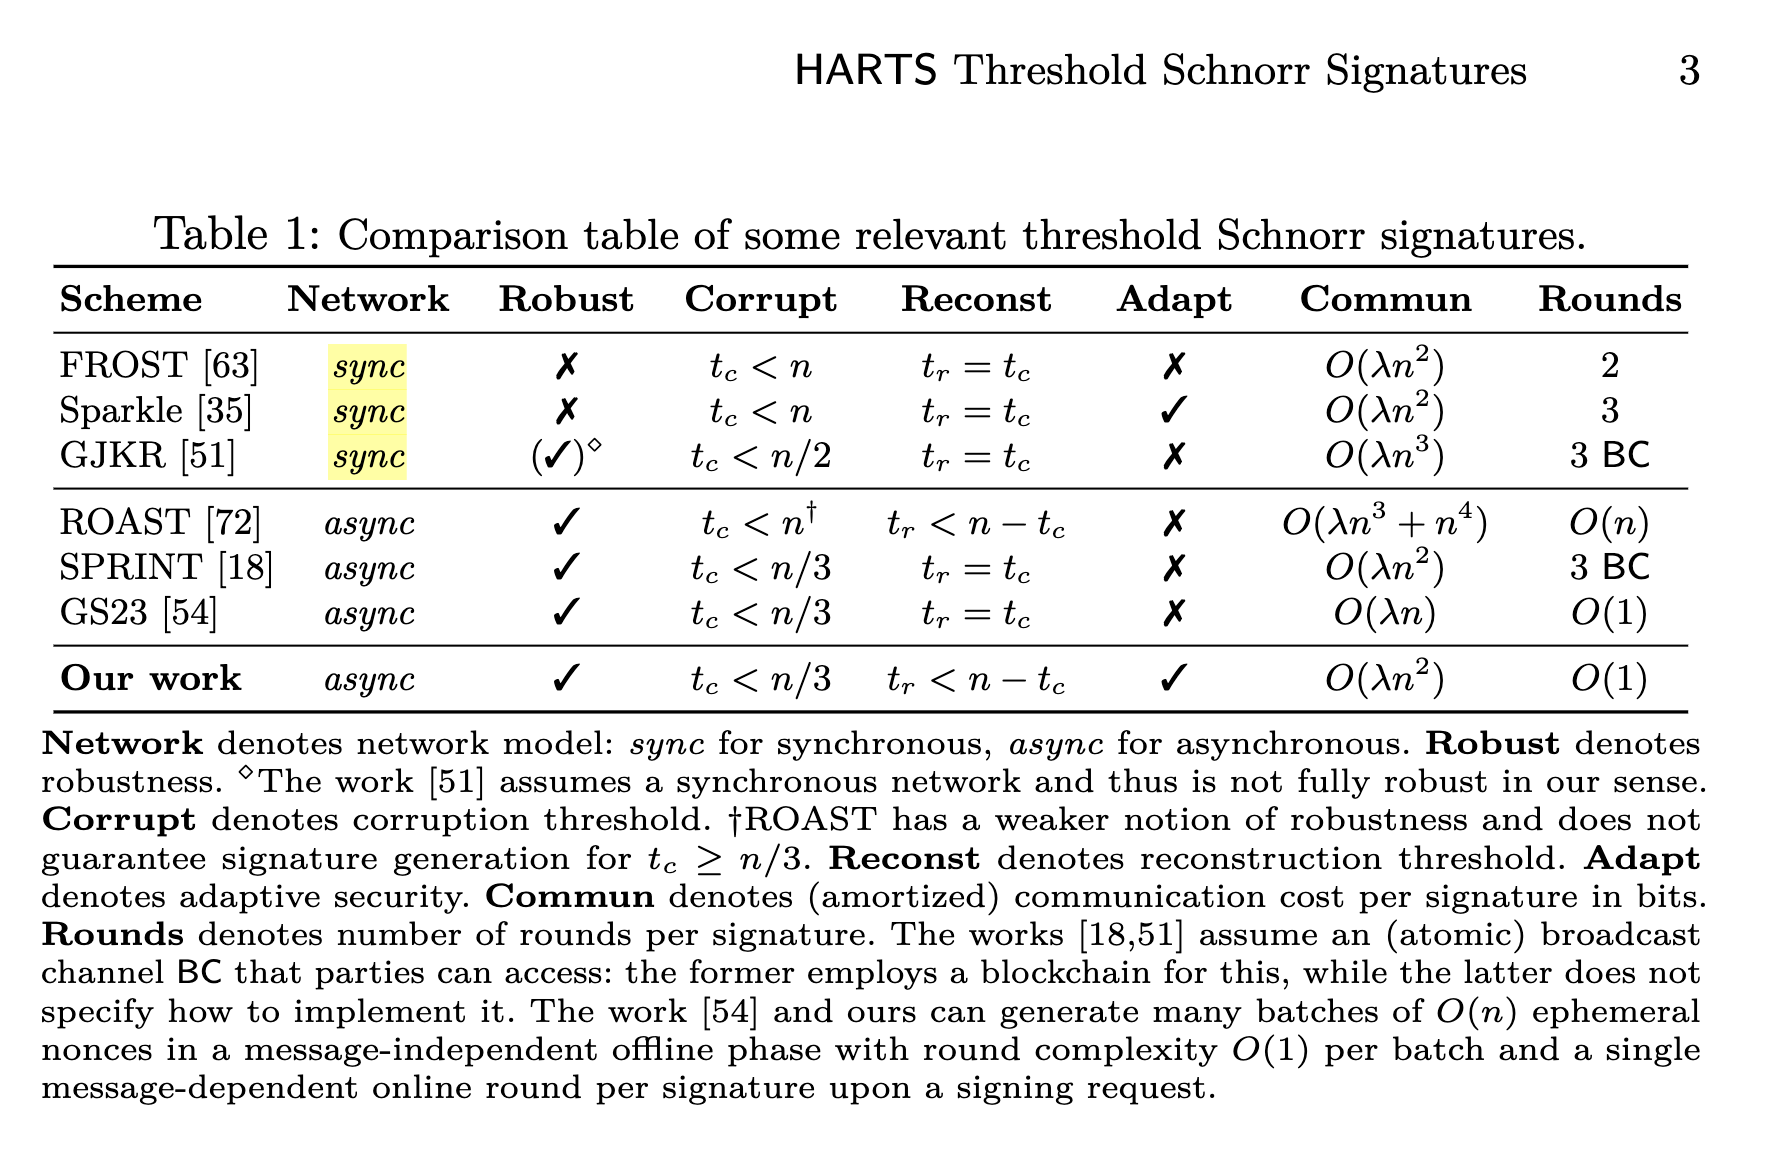
\includegraphics[width=1\linewidth]{images/HARTS_table.png}
    \caption{FROST and Sparkle are \textbf{not} forgeable in an asynchronous network, whereas GJKR is \textbf{forgeable}.}
\end{figure}

\begin{figure}
    \centering
    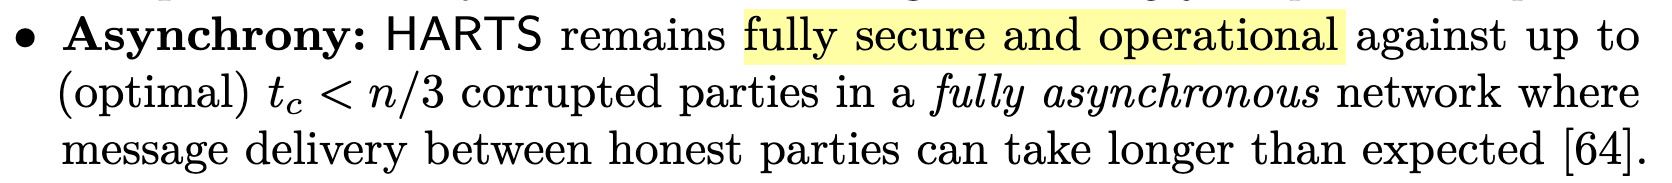
\includegraphics[width=1\linewidth]{images/HARTS_async_defn.png}
    \caption{HARTS definition of asynchrony. It is not clear what ``fully secure and operational" means.}
\end{figure}

\begin{figure}
    \centering
    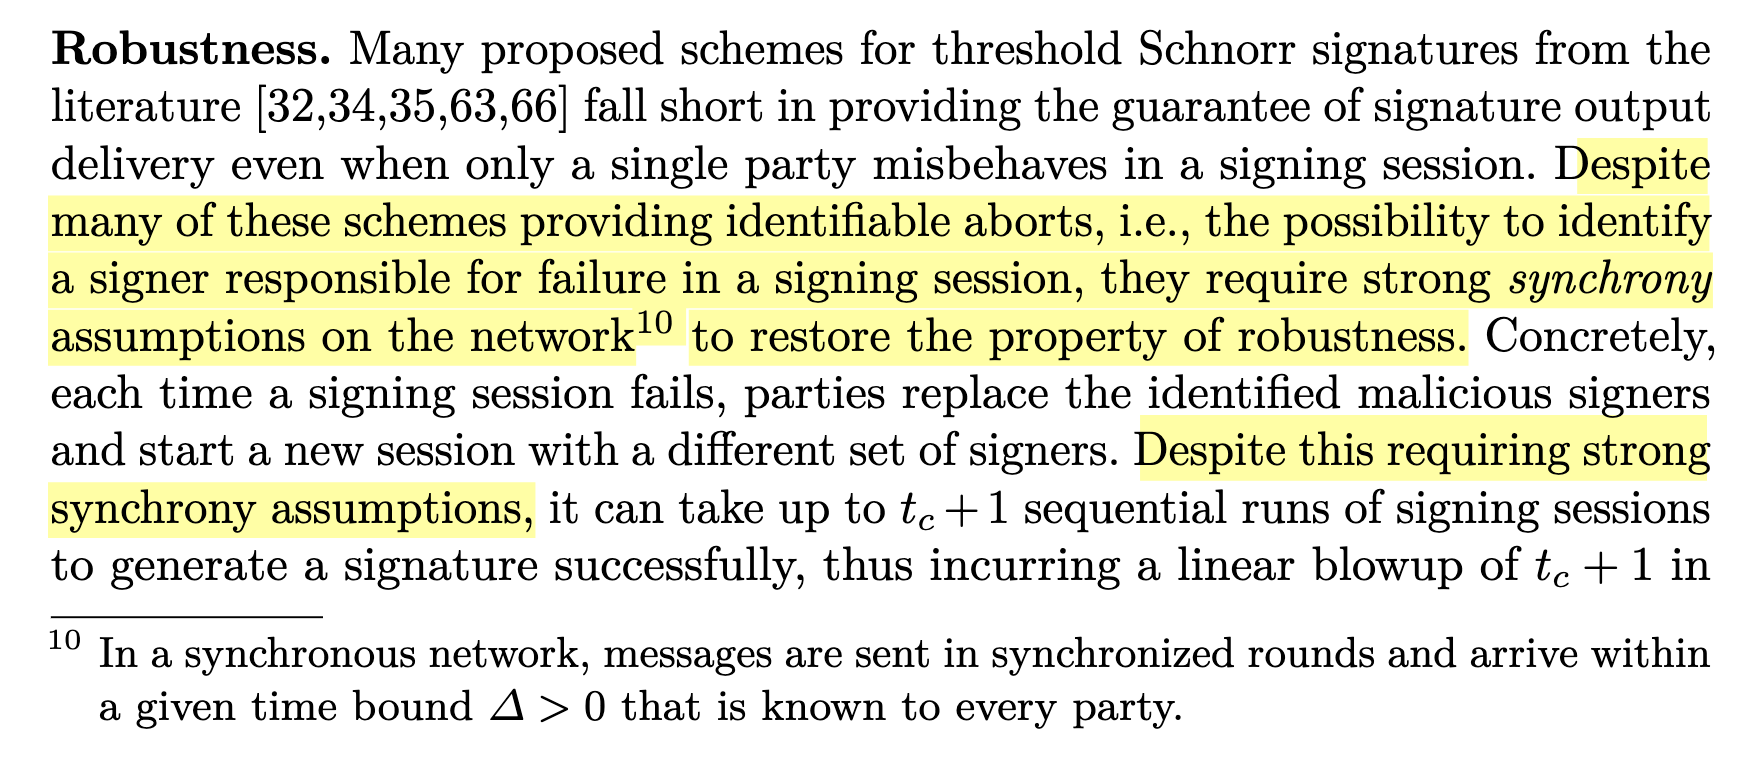
\includegraphics[width=1\linewidth]{images/HARTS_appendix.png}
    \caption{A more accurate description, buried in the appendix of HARTS, which says that synchrony is needed to restore robustness.  However, it appears to claim synchrony is needed even for just identifiable aborts.}
\end{figure}

\newpage

\subsection{SPRINT: https://eprint.iacr.org/2023/427}

\begin{figure}
    \centering
    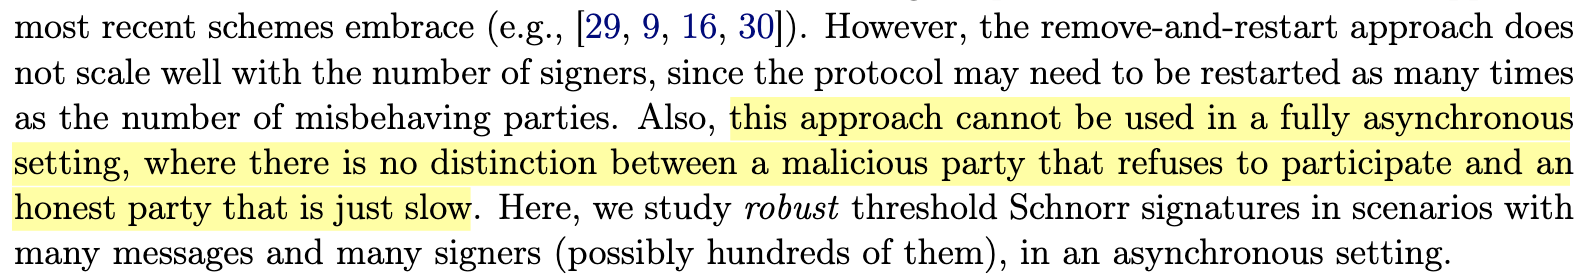
\includegraphics[width=1\linewidth]{images/SPRINT_IA.png}
    \caption{SPRINT, like HARTS, identifies synchrony as being needed for identifiable aborts.}
\end{figure}

\begin{figure}
    \centering
    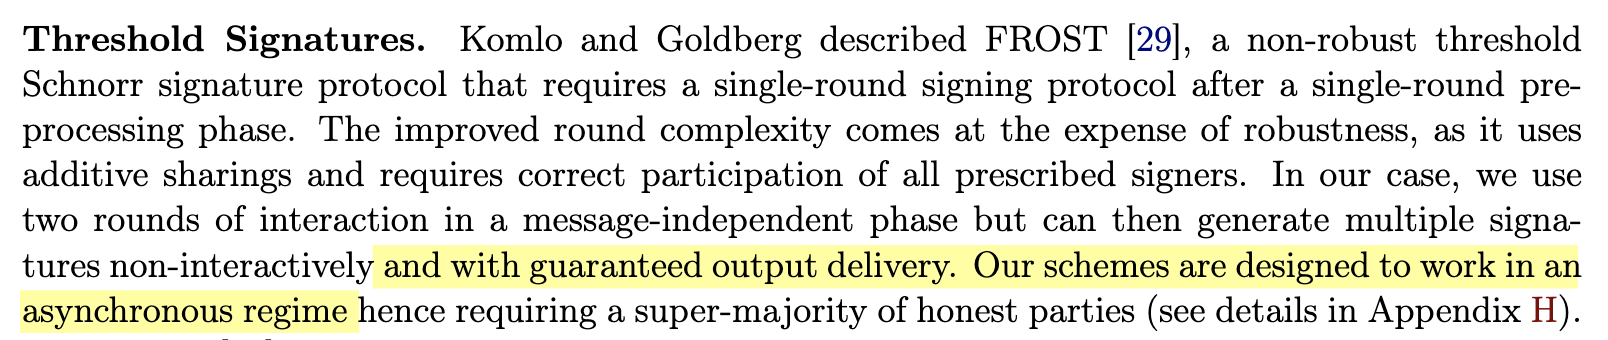
\includegraphics[width=1\linewidth]{images/SPRINT_FROST.png}
    \caption{SPRINT is a bit unclear about asynchrony.}
\end{figure}

\newpage

\subsection{ROAST: https://eprint.iacr.org/2022/550}

\begin{figure}
    \centering
    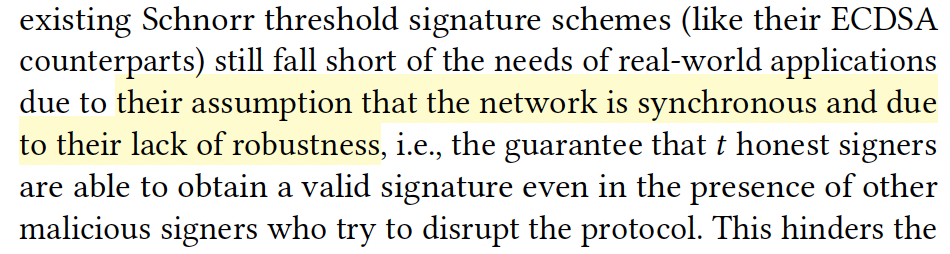
\includegraphics[width=1\linewidth]{images/ROAST_abstract.png}
    \caption{ROAST abstract says prior schemes assume synchrony.}
\end{figure}

\begin{figure}
    \centering
    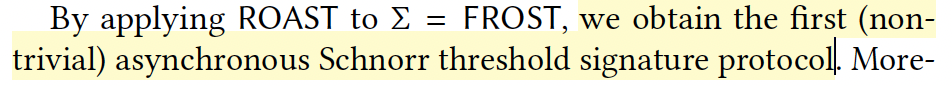
\includegraphics[width=1\linewidth]{images/ROAST_first_async.png}
    \caption{ROAST claiming to be first asynchronous threshold Schnorr scheme.}
\end{figure}

\begin{figure}
    \centering
    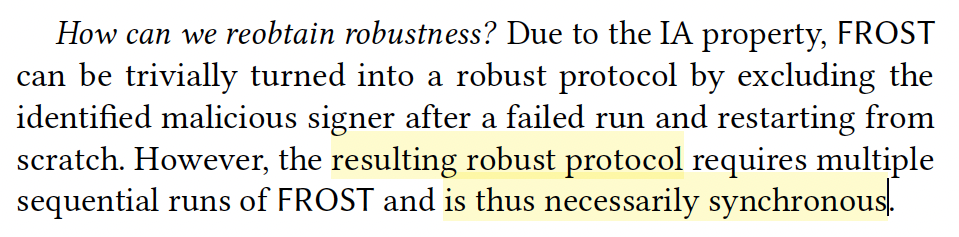
\includegraphics[width=1\linewidth]{images/ROAST_IA.png}
    \caption{Synchrony is required for the IA property of FROST.}
\end{figure}

\begin{figure}
    \centering
    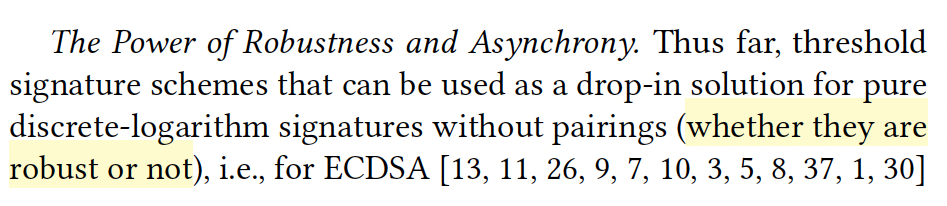
\includegraphics[width=1\linewidth]{images/ROAST_sync_reqd.png}
    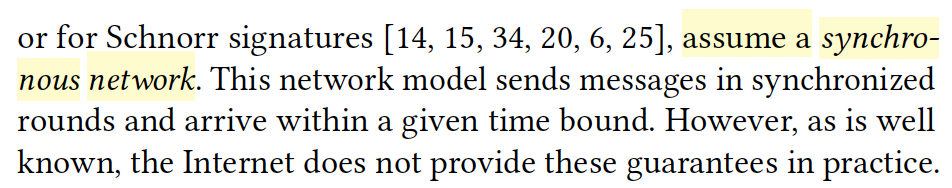
\includegraphics[width=1\linewidth]{images/ROAST_sync_reqd2.png}
    \caption{ROAST claims prior works required synchrony \textbf{whether they are robust or not}.}
\end{figure}

\begin{figure}
    \centering
    
\includegraphics[width=1\linewidth]{images/ROAST_wrapper.png}
    \caption{The trivial wrapper for FROST to make it robust is asynchronous.}
\end{figure}

\newpage

\subsection{Original FROST Paper}

\begin{figure}
    \centering
    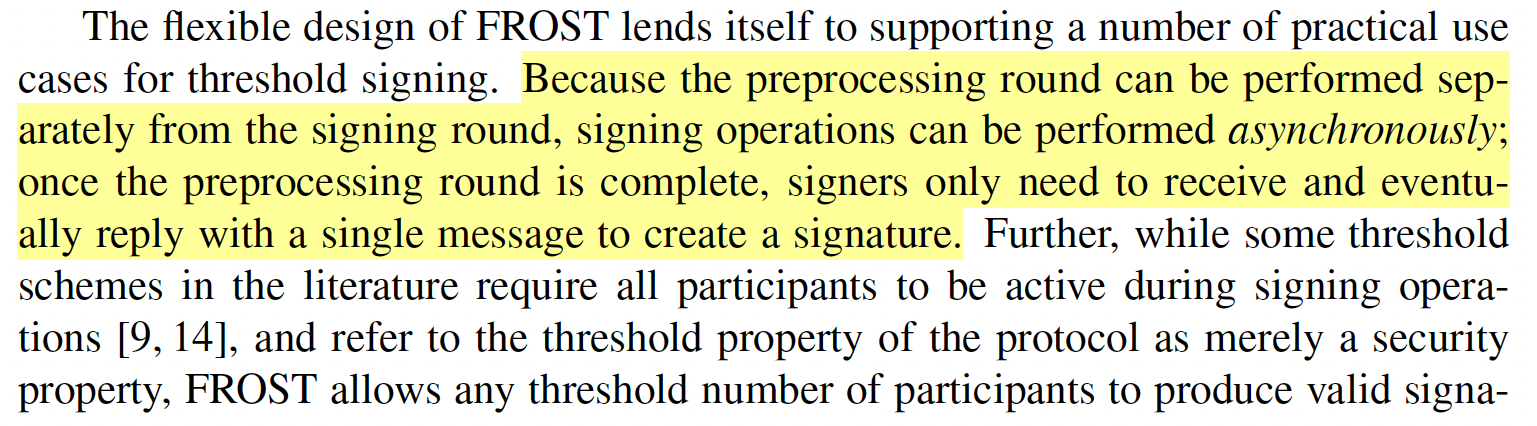
\includegraphics[width=1\linewidth]{images/FROST_async.png}
    \caption{This says only pre-processing FROST is asynchronous.}
\end{figure}

\begin{figure}
    \centering
    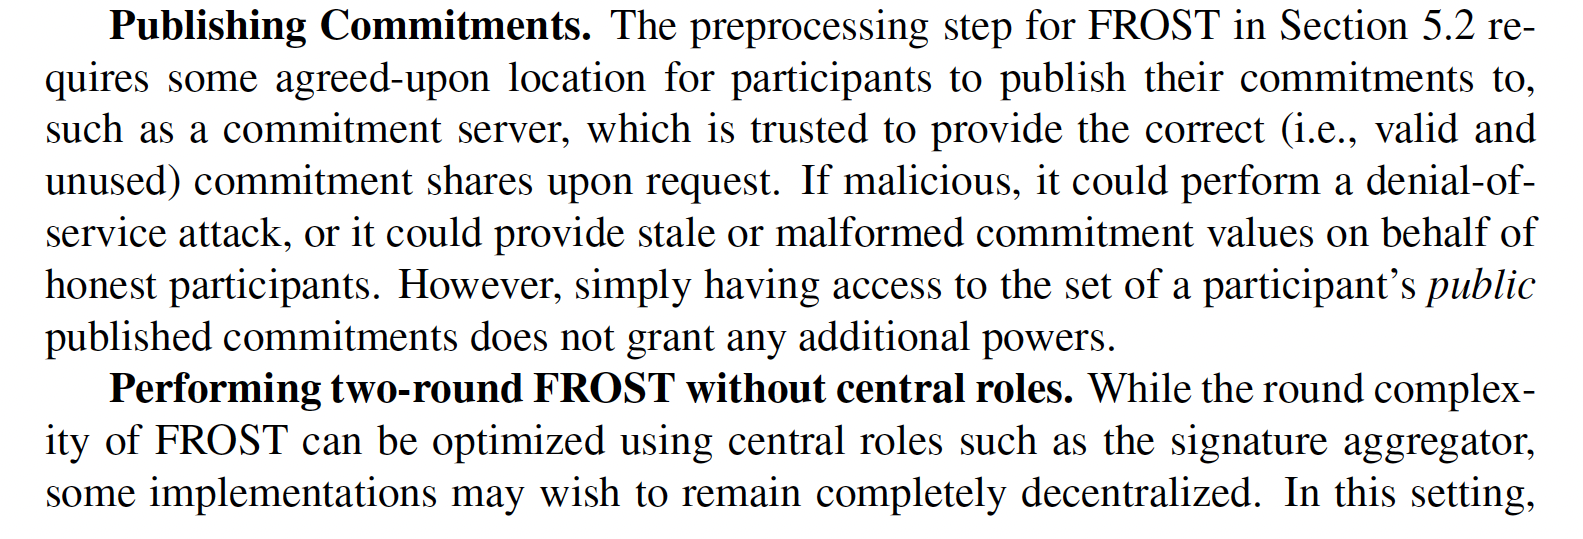
\includegraphics[width=1\linewidth]{images/FROST_aggregator.png}
    
\includegraphics[width=1\linewidth]{images/FROST_aggregator2.png}
    \caption{FROST needs to be fully two rounds if broadcast is used instead of a signature aggregator.}
\end{figure}





	%!TEX root = ../main.tex



	%!TEX root = ../main.tex

\section{Analytic complexity}\label{section:complexity}

% An analytical estimation of the (i) memory complexity, (ii) computational
% complexity, (iii) communication complexity, and (iv) round complexity of each
% proposed crypto-system. See Section 7.2 about experimental evaluation. As
% applicable, the estimates should include: a breakdown across various phases of
% the protocol; the complexity per party and for the entire system; and the
% functional dependence on configurable parameters, e.g., security strength,
% number of parties and the thresholds.

In the following sections we will refer to three phases:
\begin{itemize}
	\item "Setup" denotes any state that entities need to maintain between
	signing sessions. This is only relevant to memory complexity.
	\item "Round 1" and "round 2" denote the individual signing rounds.
\end{itemize}

We will use the following notation:
\begin{itemize}
	\item $K$: the threshold (minimum number of participants).
	\item $N$: maximum number of participants.
	\item $P$: actual number of participants.
\end{itemize}

We assume a hub-and-spoke model for the coordinator. This has the benefit of
also reflecting the analytic complexity of a protocol instantiation without a
coordinator role, in which every participant is connected to and communicating
with all other participants. In that scenario, each participant's round and
communication complexity is replaced with the coordinator's, their memory
complexity is the maximum of either, and their computational complexity is the
sum of both.

\subsection{Round complexity}

FROST requires two rounds to execute a signing session. Participants can operate
independently of each other in both rounds, and only need to communicate with
the coordinator. As such, each participant receives $1$ inbound message and
sends $1$ outbound message per round, while the coordinator correspondingly
sends $P$ outbound messages and receives $P$ inbound messages per round.

\subsection{Communication complexity}

In round 1, no information needs to be broadcast from the coordinator to
participants other than the fact that a signing round is starting. The
participants do not even learn which other participants are in the signing
session at this stage. Each participant sends back 2 encoded group elements.

In round 2, each participant receives $2P$ encoded group elements and $P$
encoded scalars, and sends back a single encoded scalar.

Communication complexity at the coordinator scales quadratically in the number
of participants: the coordinator downloads $2P$ encoded group elements at
the end of round 1, broadcasts $2P^2$ encoded group elements and $P^2$ encoded
scalars at the beginning of round 2, and downloads $P$ encoded scalars at the
end of round 2.

Note that while the coordinator sends $P$ outbound messages in round 1, the only
information that the protocol requires be conveyed is that a signing round is
starting (as noted above for participants). Empty messages are suitable for this
purpose from an analytic complexity perspective; in a real implementation there
would be some overhead due to message framing.

The information broadcast by the coordinator at the beginning of round 2 is
identical for all participants. The communication complexity at the coordinator
itself can therefore be reduced from quadratic to linear with the aid of an
authenticated broadcast channel that performs the fan-out on its behalf.
However, this shifts the quadratic cost from the coordinator to the broadcast
channel; while this may be of interest to concrete implementations, it does not
fundamentally alter the cost. Therefore for the purpose of analytic complexity
we consider the coordinator's boundary to be drawn around any broadcast channel
it may be using.

\begin{table}
	\centering
% BEGIN communication-3-5-3-128
	\begin{tabular}{c c c c}
		\toprule
		Communication & Round & Download & Upload \\ \midrule
		Coordinator & 1 & 192 & 0 \\
		            & 2 & 96 & 864 \\
		            & Total & 288 & 864 \\
		\midrule
		Participant & 1 & 0 & 64 \\
		            & 2 & 288 & 32 \\
		            & Total & 288 & 96 \\
		\bottomrule
	\end{tabular}
% END communication-3-5-3-128
	\caption{Communication complexity (in number of communicated bytes) for 3-of-5 FROST with 3 participants at the 128-bit security level.}
\end{table}

\begin{table}
	\centering
% BEGIN communication-6-10-8-224
	\begin{tabular}{c c c c}
		\toprule
		Communication & Round & Download & Upload \\ \midrule
		Coordinator & 1 & 912 & 0 \\
		            & 2 & 456 & 10944 \\
		            & Total & 1368 & 10944 \\
		\midrule
		Participant & 1 & 0 & 114 \\
		            & 2 & 1368 & 57 \\
		            & Total & 1368 & 171 \\
		\bottomrule
	\end{tabular}
% END communication-6-10-8-224
	\caption{Communication complexity (in number of communicated bytes) for 6-of-10 FROST with 8 participants at the 224-bit security level.}
\end{table}

\begin{table}
	\centering
% BEGIN communication-600-1000-700-128
	\begin{tabular}{c c c c}
		\toprule
		Communication & Round & Download & Upload \\ \midrule
		Coordinator & 1 & 44800 & 0 \\
		            & 2 & 22400 & 47040000 \\
		            & Total & 67200 & 47040000 \\
		\midrule
		Participant & 1 & 0 & 64 \\
		            & 2 & 67200 & 32 \\
		            & Total & 67200 & 96 \\
		\bottomrule
	\end{tabular}
% END communication-600-1000-700-128
	\caption{Communication complexity (in number of communicated bytes) for 600-of-1000 FROST with 700 participants at the 128-bit security level.}
\end{table}

\subsection{Memory complexity}

In the setup phase (before the start of a signing session), the coordinator and
participants need to store $N + 1$ group elements in memory, corresponding to
the group information. Participants additionally need to store 2 scalars: one
representing their identity within the signing group, and the other being their
secret share. The coordinator additionally needs to store $P$ scalars for the
identities of the signing group participants.

All of the setup data must be stored throughout the signing session, alongside
round-specific data. In the remainder of this section, as well as the tables
below, we track the "high water" mark: the maximum amount of data that the
coordinator or a participant needs to store during the round.

In round 1, the coordinator additionally stores the $2P$ encoded group elements
at the end of round 1; there is no need for these to be decoded (for validity
checking) before broadcasting them in round 2. Participants store an additional
2 group elements (along with their encodings as part of the message to the
coordinator), and 2 scalars that need to be held through the end of round 2.

In round 2, the "high water" mark for both the participants (during signing) and
the coordinator (during aggregation) is computation of the binding factors:

\begin{itemize}
	\item The hash calculation
	$\mathsf{encoded\_commitment\_hash} = \mathsf{H5}(\mathsf{encoded\_group\_commitment})$
	requires $2P$ encoded group elements and $P$ encoded scalars.
	\item The commitment list also needs to be parsed in memory for subsequent
	use, costing $2P$ group elements and $P$ scalars.
	\item The $\mathsf{H5}$ hasher stores state of at least its block size and
	output size simultaneously at some point during the calculation.
	\item The preparation of $\mathsf{rho\_input\_prefix}$ just afterwards needs
	one encoded group element and one hash output, which in the protocol
	specification are computed prior to $\mathsf{encoded\_commitment\_hash}$.
\end{itemize}

Therefore, for the protocol as specified:

\begin{itemize}
	\item The coordinator stores a maximum of $2P + N + 1$ group elements, $2P$
	scalars, $2P + 1$ encoded group elements, $P$ encoded scalars, 1 hash block,
	and 2 hash outputs in memory.
	\item Participants store a maximum of $2P + N + 3$ group elements, $P + 4$
	scalars, $2P + 1$ encoded group elements, $P$ encoded scalars, 1 hash block,
	and 2 hash outputs in memory.
\end{itemize}

An optimised implementation could reduce this maximum memory usage in several
ways:

\begin{itemize}
	\item Incrementally compute $\mathsf{encoded\_commitment\_hash}$ by updating
	the $\mathsf{H5}$ hasher with $\mathsf{encoded\_group\_commitment}$
	incrementally instead of encoding it in full.
	\item Compute the other inputs to $\mathsf{rho\_input\_prefix}$ after
	$\mathsf{encoded\_commitment\_hash}$ instead of beforehand.
\end{itemize}

\begin{table}
	\centering
% BEGIN memory-3-5-3-128
	\begin{tabular}{c c c c c c}
		\toprule
		Memory & Round & Elements & Scalars & Arb bytes & Cost \\ \midrule
		Coordinator & Setup & 6 & 3 & 0 & 672 \\
		            & 1 & 6 & 3 & 192 & 864 \\
		            & 2 & 12 & 6 & 576 & 1920 \\
		\midrule
		Participant & Setup & 6 & 2 & 0 & 640 \\
		            & 1 & 8 & 4 & 64 & 960 \\
		            & 2 & 12 & 7 & 576 & 1952 \\
		\bottomrule
	\end{tabular}
% END memory-3-5-3-128
	\caption{Memory complexity for 3-of-5 FROST with 3 participants at the 128-bit security level. The cost is in number of bytes simultaneously stored.}
\end{table}

\begin{table}
	\centering
% BEGIN memory-6-10-8-224
	\begin{tabular}{c c c c c c}
		\toprule
		Memory & Round & Elements & Scalars & Arb bytes & Cost \\ \midrule
		Coordinator & Setup & 11 & 8 & 0 & 2337 \\
		            & 1 & 11 & 8 & 912 & 3249 \\
		            & 2 & 27 & 16 & 1789 & 7318 \\
		\midrule
		Participant & Setup & 11 & 2 & 0 & 1995 \\
		            & 1 & 13 & 4 & 114 & 2565 \\
		            & 2 & 27 & 12 & 1789 & 7090 \\
		\bottomrule
	\end{tabular}
% END memory-6-10-8-224
	\caption{Memory complexity for 6-of-10 FROST with 8 participants at the 224-bit security level. The cost is in number of bytes simultaneously stored.}
\end{table}

\begin{table}
	\centering
% BEGIN memory-600-1000-700-128
	\begin{tabular}{c c c c c c}
		\toprule
		Memory & Round & Elements & Scalars & Arb bytes & Cost \\ \midrule
		Coordinator & Setup & 1001 & 700 & 0 & 118496 \\
		            & 1 & 1001 & 700 & 44800 & 163296 \\
		            & 2 & 2401 & 1400 & 67488 & 342784 \\
		\midrule
		Participant & Setup & 1001 & 2 & 0 & 96160 \\
		            & 1 & 1003 & 4 & 64 & 96480 \\
		            & 2 & 2401 & 704 & 67488 & 320512 \\
		\bottomrule
	\end{tabular}
% END memory-600-1000-700-128
	\caption{Memory complexity for 600-of-1000 FROST with 700 participants at the 128-bit security level. The cost is in number of bytes simultaneously stored.}
\end{table}

\subsection{Computational complexity}

The coordinator performs no significant computations in round 1. Participants
perform 2 fixed-base exponentiations, and (for the security levels presented in
this document) process 2 blocks of hash function input.

The significant computations occur during round 2.

Participants perform $2P$ group element multiplications, $P$ exponentiations,
$P + 1$ scalar additions, and $2P + 2$ scalar multiplications. The during
aggregation, the coordinator performs $2P$ group element multiplications, $P$
exponentiations, and $P$ scalar additions.

TODO: Fill out hash function complexity.

TODO: Convey the multi-exp by showing the number of terms in it, and then include
its muls etc. for a specific algorithm in the table (e.g. Pippenger).

\begin{table}
	\centering
% BEGIN computational-3-5-3-128
	\begin{tabular}{c c c c c c c c c c c c c}
		\toprule
		Computation & Round & $\mathsf{Read}_A$ & $\mathsf{Write}_A$ & $A \times A$ & $A^k$  & $B^k$  & $\mathsf{Read}_k$ & $\mathsf{Write}_k$ & $k + k$ & $k \times k$ & $k^n$ & H blocks \\ \midrule
		Coordinator & 1 & 0 & 0 & 0 & 0 & 0 & 0 & 0 & 0 & 0 & 0 & 0 \\
		            & 2 & 6 & 7 & 6 & 3 & 0 & 3 & 15 & 3 & 0 & 0 & 10 \\
		            & Total & 6 & 7 & 6 & 3 & 0 & 3 & 15 & 3 & 0 & 0 & 10 \\
		\midrule
		Participant & 1 & 0 & 2 & 0 & 0 & 2 & 0 & 2 & 0 & 0 & 0 & 2 \\
		            & 2 & 6 & 9 & 6 & 3 & 0 & 3 & 7 & 4 & 8 & 1 & 11 \\
		            & Total & 6 & 11 & 6 & 3 & 2 & 3 & 9 & 4 & 8 & 1 & 13 \\
		\bottomrule
	\end{tabular}
% END computational-3-5-3-128
	\caption{Computational complexity for 3-of-5 FROST with 3 participants at the 128-bit security level.}
\end{table}

\begin{table}
	\centering
% BEGIN computational-6-10-8-224
	\begin{tabular}{c c c c c c c c c c c c c}
		\toprule
		Computation & Round & $\mathsf{Read}_A$ & $\mathsf{Write}_A$ & $A \times A$ & $A^k$  & $B^k$  & $\mathsf{Read}_k$ & $\mathsf{Write}_k$ & $k + k$ & $k \times k$ & $k^n$ & H blocks \\ \midrule
		Coordinator & 1 & 0 & 0 & 0 & 0 & 0 & 0 & 0 & 0 & 0 & 0 & 0 \\
		            & 2 & 16 & 17 & 16 & 8 & 0 & 8 & 80 & 8 & 0 & 0 & 36 \\
		            & Total & 16 & 17 & 16 & 8 & 0 & 8 & 80 & 8 & 0 & 0 & 36 \\
		\midrule
		Participant & 1 & 0 & 2 & 0 & 0 & 2 & 0 & 2 & 0 & 0 & 0 & 2 \\
		            & 2 & 16 & 19 & 16 & 8 & 0 & 8 & 17 & 9 & 18 & 1 & 37 \\
		            & Total & 16 & 21 & 16 & 8 & 2 & 8 & 19 & 9 & 18 & 1 & 39 \\
		\bottomrule
	\end{tabular}
% END computational-6-10-8-224
	\caption{Computational complexity for 6-of-10 FROST with 8 participants at the 224-bit security level.}
\end{table}

\begin{table}
	\centering
% BEGIN computational-600-1000-700-128
	\begin{tabular}{c c c c c c c c c c c c c}
		\toprule
		Computation & Round & $\mathsf{Read}_A$ & $\mathsf{Write}_A$ & $A \times A$ & $A^k$  & $B^k$  & $\mathsf{Read}_k$ & $\mathsf{Write}_k$ & $k + k$ & $k \times k$ & $k^n$ & H blocks \\ \midrule
		Coordinator & 1 & 0 & 0 & 0 & 0 & 0 & 0 & 0 & 0 & 0 & 0 & 0 \\
		            & 2 & 1400 & 1401 & 1400 & 700 & 0 & 700 & 491400 & 700 & 0 & 0 & 1927 \\
		            & Total & 1400 & 1401 & 1400 & 700 & 0 & 700 & 491400 & 700 & 0 & 0 & 1927 \\
		\midrule
		Participant & 1 & 0 & 2 & 0 & 0 & 2 & 0 & 2 & 0 & 0 & 0 & 2 \\
		            & 2 & 1400 & 1403 & 1400 & 700 & 0 & 700 & 1401 & 701 & 1402 & 1 & 1928 \\
		            & Total & 1400 & 1405 & 1400 & 700 & 2 & 700 & 1403 & 701 & 1402 & 1 & 1930 \\
		\bottomrule
	\end{tabular}
% END computational-600-1000-700-128
	\caption{Computational complexity for 600-of-1000 FROST with 700 participants at the 128-bit security level.}
\end{table}

	\section{Deployment Recommendations}\label{section:deployment-recommendations}

% A set of deployment requirements and recommendations, including those
% related to security. This section should also include a list of known and
% proposed applications of the submitted threshold scheme(s).

\subsection{Key Share Storage}

Participants should store their key shares securely, following common secure
practice to store secrets, such as making them readable only by the owner and
storing them encrypted by the operating system keyring or keychain.

Note that it is technically possible for a participant to recover a lost share
with the help of a threshold of other participants. However, this feature is
not covered by this submission.


\subsection{Managing State}

As detailed in Section~\ref{section:comparisons:statemanagement} participants must
manage some state. In each FROST signing session, the participant must keep the
nonces generated in the first round 1, which will be then read again in round 2.
It is recommended that each signing session be assigned some sort of unique
random session ID, so that each participant can map between the session ID and
the nonces for that session. Additionally, nonces should be deleted after they
are used. It is not recommended to persist nonces in long term storage unless
strictly necessarily, to avoid the risk of accidental nonce misuse.

\subsection{Communication Channels}

FROST does not require authenticated nor encrypted channels, as detailed
in Section~\ref{section:system-model}. However, authentication allows identifiable
aborts, which allow pinpointing participants who are not following the protocol
correctly; this can allow the exclusion of that participant for further signing
rounds. Additionally, we expected that encrypted channels might be desired in
many applications due to the private nature of messages being signed.

To authenticate and possibly encrypt communications, we recommend that each
participant should be issued a ``communication keypair'', and each participant
must verify each other's communication public key by some out of band method.
These keypairs can then bootstrap the authenticated and encrypted channels by
using some cryptographic mechanism. We suggest using the Noise protocol (TODO:
ref), specifically the one-way ``X'' pattern which will not add additional
rounds to the FROST protocol. If higher security assurances are needed (such as
stronger forward secrecy), then the ``XK'' pattern might be used, but it adds an
additional round between participants and coordinator to complete the Noise
handshake.

\subsection{Known and Proposed Applications}

It's worth pointing out that most of the proposed applications are not specific
to FROST and could be accomplished by similar threshold signature schemes.

\begin{description}
    \item[Certificate Authorities.] Certificate issuers can use FROST to protect
    issuance keys and make it harder for attackers to compromise a certificate
    authority.
    \item[Legally Binding Eletronic Signatures.] Many jurisdictions allow the
    possibility of using electronic signatures to sign documents. FROST can
    offer an alternative to help secure the critically important private key,
    without needing to resort to self-managed hardware tokens or
    externally-hosted keys inside hardware security modules.
    \item[Cryptocurrency Wallets.] Wallets can use FROST to make them more
    resilient to hacking. FROST is also useful for scenarios where an
    organization need to manage a cryptocurrency wallet with the organization
    funds and multiple persons are required to sign off on spends.
    \item[Cryptocurrency Bridges.] Automated bridges which convert between
    different cryptocurrencies can be built using FROST, where multiple
    distributed nodes manage bridged funds and can issue transfer in response
    to claims for the bridged currency.
    \item[Code Signing.] In many scenarios, such as publishing an app to an
    application store or publishing a software package to a package repository,
    the authenticity of software is guaranteed by a digital signature. Thus, the
    digital signature controls the distribution of software to million of users,
    and ensuring the security of the underlying private key is crucial to
    prevent bad actors from publishing compromised version of those software.
    FROST can help protecting that private key.
    \item[WebAuthn.] The WebAuthn standard specifies mechanisms for
    authenticating users into applications and services. FROST could help
    protect the underlying private key for security-critical credentials.
\end{description}


	\printbibliography


  %\appendix

\end{document}
